\section{12.8 Metoda kolejnych nadrelaksacji - SOR (succesive overrelaxation)}

\begin{frame}{Metoda kolejnych nadrelaksacji - SOR (succesive overrelaxation)}
  Inaczej zapisany wzór roboczy SR(G-S):
$$x^{(t+1)}_{i}=x^{(t)}_{i} \underbrace{\frac{1}{a_{ii}}[b_i-\sum^{i-1}_{j/1} a_{ij} x^{(t+1)}_j -\sum^{n}_{j/1} a_{ij} x^{(t)}_j ]}_{r^{(t)}_i \text{- poprawka do staregio rozwiązania } x^{(t)}_i}$$
  %stare roziwązanie? poprawione z śtaregożozwiazania
  Przyspieszenie zbieżności:
  $$\boxed{x^{(t+1)}_{i}=x^{(t)}_{i}+\omega r^{(t)}_{i}}, \text{$\omega$ - pewna liczba}$$
\end{frame}

\begin{frame}
  wzór roboczy
  $$a_{ii}x^{(t+1)}_{i}=\underbrace{a_{ii}}_{\Delta}x^{(t)}_{i}+\omega[b_i-\sum^{i-1}_{k/1}a_{ij}x^{(t+1)}_{j}-\sum^{n}_{j/i+1}a_{ij}x^{(t)}_{j}]-\omega\underbrace{a_{ii}}_{\Delta}x^{(t)}_{i}$$
  w zapisie macierzowym
  $$Dx^{(t+1)}=(1-\omega )Dx^{(t)}+\omega [b-Lx^{(t+1)}-Ux^{(t)}]$$
  po uporządkowaniu:
  $$x^{(t+1)}=\underbrace{(D+\omega L)^{-1}[I-\omega (D+U)]}_{M}x^{(t)}+\underbrace{\omega(D+\omega L)^{-1}b}_{W(=B^{-1}b)}$$
\end{frame}

\begin{frame}{}
  \textbf{Twierdzenie}
  \begin{block}{Założenia}
    Dla dowolnej nieosobliwej macierzy A i dowolnej liczby $\omega$ zachodzi:
  \end{block}
  \begin{block}{Teza}
    $$\rho(M)\geq |\omega -1|$$
    Stąd:
    $$
    \omega\in(0,2) \Rightarrow
    \begin{cases}
      \omega\in{(0,1]}\text{\quad- podrelaksacja}\\
      \omega\in{(1,2)}\text{\quad- nadrelaksacja}
    \end{cases}
    $$
  \end{block}
\end{frame}

\begin{frame}{}
  interpretacja:
  Dla ważnych praktycznie klas macierzy znana jest optymalna wartość $\omega$
  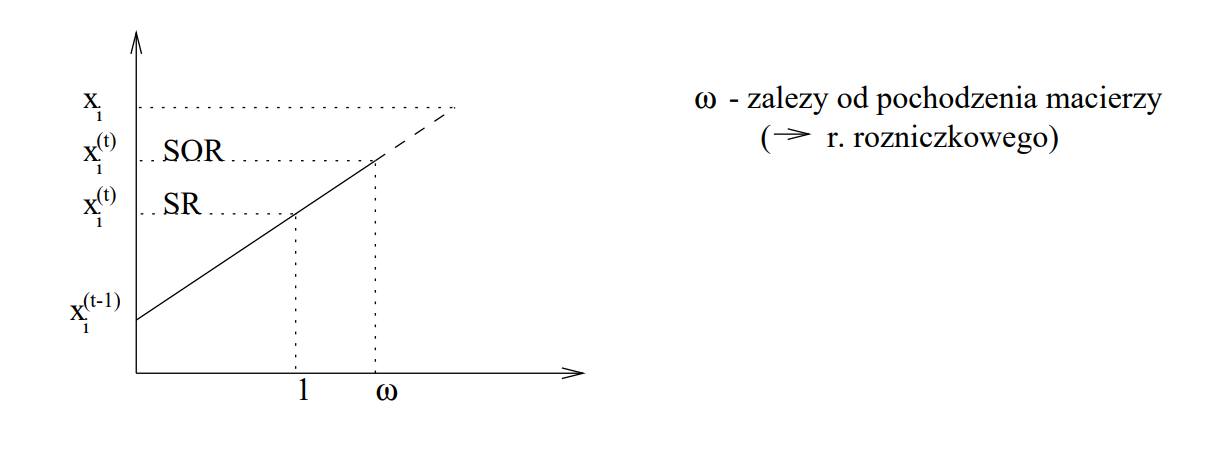
\includegraphics[height=0.6\textheight, width=1\textwidth]{img/12/iteracja2}
\end{frame}

\begin{frame}{}
  \textbf{Twierdzenie}
  \begin{block}{Założenia}
    Dla A - symetrycznej, dodatnio określonej o postacji blokowo - trójprzekątniowej:
    $$
    A=\begin{bmatrix}
    D_1 & U_1 &&&&\\
    L_2 & D_2 & U_2 &&& \\
    &&...&...&&\\
    &&&L_{n-1}&D_{n-1}&U_{n-1}\\
    &&&&L_n&D_n
    \end{bmatrix}
    $$
  \end{block}
\end{frame}

\begin{frame}
  \begin{block}{Teza}
    $$\rho(M_{GS})=\rho^2(M_J)$$
    $$\omega_{opt}=\frac{2}{1+sqrt{1-\rho(M_{GS})}}$$
    $$\lambda_{SOR}=\omega_{opt}-1$$
  \end{block}
  \begin{exampleblock}{Dla równania modelowego}
    $$\rho=cos^2(\frac{\pi}{N}), \omega_{opt}\approx2(1-\frac{\pi}{N}, \lambda_{SOR}=1-\frac{2\pi}{N}$$
  \end{exampleblock}
\end{frame}


